\section{Character encodings and glyphs}\label{section:unicode}
\label{sec:charsets}
\epigraph{Thou whoreson zed, thou unnecessary letter!}{Wiliam Shakespeare, \textit{King Lear}}

We'll be well-served by becoming familiar with our core building
blocks---character sets and their rasterized forms. Even if we were to shrink
the character cell to a single pixel, we'd still need write one or another
character into it, and emit a control code to stylize it\footnote{I've seen
this idea bandied about as if it's a serious suggestion. Besides the fact
that it won't work in a console, escapes are \textit{far} less efficient than
canvases or OpenGL display lists; if your plan involves using ANSI escape
sequences to drive a 1920x1080 display via roughly two million 1x1 character
cells, you're not going to space today, or maybe ever\cite{upgoerfive}.}.

In the beginning, there are somewhat Platonic \textit{characters}, one of the
most imprecise terms in all of computer science (even when we leave aside the
data type \texttt{char}). In and of itself, a character is nothing more than an
identifier: \texttt{LATIN CAPITAL LETTER I}\footnote{Isn't that a recursive
definition? You betcha.}. There are many things a character is not:

\begin{denseitemize}
\item{A character is not necessarily unique within a character set (see diacritic vs.\ precomposed forms).}
\item{Different characters needn't be distinct glyphs\cite{nothinggoesaway}.}
\item{A character needn't limit itself to a single column, even when using a fixed-width font.}
\item{A character does not necessarily have a visual representation.}
\item{A character does not necessarily have a single meaning among different languages.}
\item{In a given encoding, all characters are not necessarily the same size.}
\item{A character cannot necessarily capture the state of the keyboard at some time.}
\item{A character cannot necessarily describe a cell of a display at some time.}
\end{denseitemize}

Collecting characters and assigning them distinct (but not necessarily contiguous)
numbers creates a \textit{code set}, and the smallest contiguous
range of numbers covering this code set is a \textit{code space}. The Unicode 13
code space is comprised of 17 contiguous planes of 65,536 code points each, for
a size of $17*2^{16}$. It defines 143,859 characters, smaller than its
code space by an order of magnitude. A map from a code set to a set of bit
sequences is a \textit{character encoding}. There are numerous standard
encodings of the Universal Character Set, each of which represents the entire
set in different ways (the best one is UTF-8, as we will see). Character sets
are registered with IANA per RFC 2978\cite{rfc2978}, and character encodings
are registered with the ISO Register of Coded Characters per ISO/IEC 2375\cite{iso2375}.

Character graphics are formed from \textit{glyphs}, the visual renderings of a
character encoding, supplied by a font. These glyphs might fuse into what
Unicode Standard Annex \#29\cite{annex29} refers to as a \textit{user-perceived
character} or \textit{grapheme cluster}. A formal algorithm for dividing a
stream of glyphs into grapheme clusters (``horizontally segmentable units of
text\cite{meaningcodepoints}'') achieves \textit{segmentation}. The current
Unicode segmentation algorithm yields \textit{extended grapheme clusters}.

These extended grapheme clusters (EGCs) can be thought of as the atoms of
character graphics. It is not generally possible to write them partially, nor
to partially overlay one atop another. Backspacing ought usually remove entire EGCs
at a time. The cursor ought cross an EGC in a single movement. In Notcurses,
each cell of a plane can hold a single EGC, which must be written as a single
unit. The actual number of columns occupied by an EGC is a property of the font
and layout engine being used.

In the modern era, Unicode is used just about everywhere, and programs must be
prepared to handle it. On the plus side, Unicode presents a single, coherent
means of representing all the world's languages, eliminating the old necessity
of switching among encodings at runtime. UNIX has its origins---and most of its
modern UI---in a much smaller character set: ASCII.

\subsection{Everyone loves ASCII}
\begin{wrapfigure}{o}{.5\textwidth}
  \fbox{%
    \parbox{0.5\textwidth}{
In the early 1960s, an IBM employee on a dare ate a hallucinogenic tapeworm
that pissed nitric acid. Stuffing his steaming, rapidly decoiling bowels
up into a brown paper bag, he was off to the hospital. Alas! On those very
hospital steps he was struck by lightning, and trepanned with great drills, and
set upon by savage hogs, and finally exploded. The tapeworm emerged, clad
in shimmering mandorla, with a name pronounceable by no human tongue. ``Adding
hallucinogenic tapeworms to a late project only makes it later,'' cautioned Fred
Brooks\cite{mythicalman}, but Gene Amdahl knew no peace. ``This
Tapeworm Queen reminds me of halcyon Wisconsin days!'' he cried, and on a prototype
Model 30 appeared her Name. Struck by the power of that Name, all began to bow,
and to weep. She vomited forth the Tapeworm Gospel. Looking upon this filth, they
thought it Good.\\
So now you know what EBCDIC is. There ended up being no fewer than 57
variants\cite{searle} of EBCDIC, worthy of Heinz. We will speak of it no
further. If you find yourself needing more information about EBCDIC, think long
and hard about your life decisions.}%
  }
\end{wrapfigure}
The first digital codes were the English telegraph system of Charles Wheatstone
and William Cooke, and American Samuel Morse's code, with which he in 1837 famously
signaled ``What hath God wrought!'' The Morse system was simpler, running
over a single line, and quickly won out. The teleprinter of Jean-Maurice-Émile Baudot
(from whom we derive the modern unit \textit{baud}) followed in
1874\cite{evolutioncodes}, with its pentabit, fixed-length Baudot code. Baudot
code required 7.42 bittimes per character; at a typical 0.022s bittime, it
could transmit just over 6 characters per second\cite{martin}.

For our purposes, the story can reasonably start with a 7-bit encoding of
128 characters: ANSI X3.4-1986, perhaps better known as ASCII (Table~\ref{table:ascii}).
The first ASCII we would recognize as such\footnote{To paraphrase G.\ H.\
Hardy, ``ASCII-1963 was clever schoolboys; '68 a Fellow from another
College\cite{ghhardy}.''} was the unpublished ASCII-1965. The ASA (ANSI
before it was ANSI) ASCII 1963 didn't even have minuscules\footnote{Uppercase
and lowercase are loanwords from printing, where the two sets were
stored in different cases of the typesetting table. ``Majuscules'' and
``minuscules'' will mark your good breeding.}. ASCII-1968 was
released as USAS X3.4-1968 to wild acclaim. The ISO/IEC 646 standard\cite{iso646}
``internationalized'' ASCII-1968 by opening up 12 graphic characters to
regional specifications (the US ASCII defined the ``International Reference
Variant'')\cite{aivosto}.

The first 32 values are non-printable control codes, first given their current
definitions in ASCII 1968. These 32 codes (known as the ``C0'' coded control
set since ISO/IEC 646) lived on through ISO/IEC 2022 (ECMA-35), ISO/IEC 6429
(ECMA-48), and ISO/IEC 8859 (ECMA-94), and are reproduced in today's ISO/IEC 10646,
aka the Universal Character Set. They're common across just about every
character set of which I'm aware (EBCDIC went almost entirely its own way,
because EBCDIC), despite being largely archaic and altogether mystifying. Most
of the associated semantics have been obsoleted, and in some cases the encoded
characters are now used for different purposes than originally planned (see
Table~\ref{table:c0maps}). These characters can be entered by pressing Ctrl
along with another key from ASCII; these combinations are defined using
``caret notation''.

\begin{table}[!htb]
  \centering
  \texttt{%
  \begin{tabular}{ |c||c|c|c|c|c|c|c|c|c|c|c|c|c|c|c|c|c| }
    \hline
    & x0 & x1 & x2 & x3 & x4 & x5 & x6 & x7 & x8 & x9 & xa & xb & xc & xd & xe & xf \\
    \hline
    \hline
    0x & NUL & SOH & STX & ETX & EOT & ENQ & ACK & BEL & BS & HT & LF & VT & FF & CR & SO & SI \\
    \hline
    1x & DLE & DC1 & DC2 & DC3 & DC4 & NAK & SYN & ETB & CAN & EM & SUB & ESC & FS & GS & RS & US \\
    \hline
    2x & SP & ! & " & \cellcolor{blue!25}\# & \cellcolor{blue!25}\$ & \% & \& & ' & ( & ) & * & + & , & - & . & / \\
    \hline
    3x & 0 & 1 & 2 & 3 & 4 & 5 & 6 & 7 & 8 & 9 & : & ; & < & = & > & ? \\
    \hline
    4x & \cellcolor{blue!25}@ & A & B & C & D & E & F & G & H & I & J & K & L & M & N & O \\
    \hline
    5x & P & Q & R & S & T & U & V & W & X & Y & Z & \cellcolor{blue!25}[ & \cellcolor{blue!25}\textbackslash{} & \cellcolor{blue!25}] & \cellcolor{blue!25}\^{} & \_ \\
    \hline
    6x & \cellcolor{blue!25}\textasciigrave{} & a & b & c & d & e & f & g & h & i & j & k & l & m & n & o \\
    \hline
    7x & p & q & r & s & t & u & v & w & x & y & z & \cellcolor{blue!25}\{ & \cellcolor{blue!25}| & \cellcolor{blue!25}\} & \cellcolor{blue!25}\textasciitilde{} & DEL \\
    \hline
  \end{tabular}
  }
  \caption[ANSI X3.4-1986 (ASCII)]{ANSI X3.4-1986 (ISO/IEC 646-IRV, IA5, T.50 IRA, RFC 20)---American Standard Code for Information Interchange. Shaded characters can be replaced in regional variants.}
  \label{table:ascii}
\end{table}

Recall the \texttt{struct termios} from Chapter~\ref{section:tty}. The \texttt{c\_cc}
array of that structure defines ``special characters'' for the terminal. Aside from
CR and LF, the various caret controls can there be recovered and redefined. Should
you really want to send \texttt{SIGINT} via 'a' rather than Ctrl+C, that's where
you can do it.

\begin{table}[!htb]
  \centering
  \begin{tabular}{ |c|c|c|c|l| }
    \hline
    Character & Caret & C & \texttt{c\_cc} & Semantics \\
    \hline
    \hline
    0x00 (NUL) & \texttt{\^{}@} & & & \\
    \hline
    0x03 (ETX) & \texttt{\^{}C} & & \texttt{VINTR} & Deliver \texttt{SIGINT} \\
    \hline
    0x04 (EOT) & \texttt{\^{}D} & & \texttt{VEOF} & Indicate end-of-file \\
    \hline
    0x07 (BEL) & \texttt{\^{}G} & \textbackslash{}a & & Alert (bell) \\
    \hline
    0x08 (BS) & \texttt{\^{}H} & \textbackslash{}b & & Backspace \\
    \hline
    0x09 (HT) & \texttt{\^{}I} & \textbackslash{}t & & Proceed to next tab stop \\
    \hline
    0x0a (LF) & \texttt{\^{}J} & \textbackslash{}n & & Move down one line \\
    \hline
    0x0b (VT) & \texttt{\^{}K} & \textbackslash{}v & & Move down to next vertical tab \\
    \hline
    0x0c (FF) & \texttt{\^{}L} & \textbackslash{}f & & Move to start of line \\
    \hline
    0x0d (CR) & \texttt{\^{}M} & & & Carriage return \\
    \hline
    0x0e (SO) & \texttt{\^{}N} & & & (ISO 2022 mode) SO/LS1 \\
    \hline
    0x0f (SI) & \texttt{\^{}O} & & \texttt{VDISCARD} & (ISO 2022 mode) SI/LS0 \\
    \hline
    0x11 (DC1) & \texttt{\^{}Q} & & \texttt{VSTART} & Software flow control (resume output) \\
    \hline
    0x12 (DC2) & \texttt{\^{}R} & & \texttt{VREPRINT} & Reprint input prompt \\
    \hline
    0x13 (DC3) & \texttt{\^{}S} & & \texttt{VSTOP} & Software flow control (pause output) \\
    \hline
    0x15 (NAK) & \texttt{\^{}U} & & \texttt{VKILL} & Erase line \\
    \hline
    0x16 (SYN) & \texttt{\^{}V} & & \texttt{VLNEXT} & Literal next---inhibit translation\\
    \hline
    0x17 (ETB) & \texttt{\^{}W} & & \texttt{VWERASE} & Erase word \\
    \hline
    0x1a (SUB) & \texttt{\^{}Z} & & \texttt{VSUSP} & Deliver \texttt{SIGTSTP} \\
    \hline
    0x1b (ESC) & \texttt{\^{}[} & & & Initiate escape sequence \\
    \hline
    0x1c (FS) & \texttt{\^{}\textbackslash{}} & & \texttt{VQUIT} & Deliver \texttt{SIGQUIT} \\
    \hline
    0x1d (GS) & \texttt{\^{}]} & & & \\
    \hline
    0x1e (RS) & \texttt{\^{}\^{}} & & & \\
    \hline
    0x1f (US) & \texttt{\^{}\_} & & & \\
    \hline
  \end{tabular}
  \caption[Usual UNIX semantics of C0]{Usual UNIX semantics of C0. The exact mappings can be inspected with \texttt{stty -a}.}
  \label{table:c0maps}
\end{table}

From Table~\ref{table:c0maps}, it should be obvious that Ctrl essentially clears
the top two bits of a 7-bit ASCII input. It might be less obvious that all
minuscules are equal to the sum of 0x20 and their corresponding majuscule,
allowing lowercase and uppercase to be switched by toggling the fifth (32) bit.
Likewise, 0xDF provides a fast case-insensitive eight-bit comparison mask (it
is necessary to mask out 0x2). Numeric values
for a digit can be acquired by subtracting 0x30 ('0'). Printable characters are all
those with a 1 in any of the higher five bits, save 0x7F\footnote{Why 0x7f? Like
so many things, this comes down to punch cards. If you've punched an error on
a group of 7 holes, and want to correct it, what are your choices? The only
general solution is to interpret all 7 holes as a strikeout\cite{cardpunch}.}. Numeric values for a
letter can be acquired by subtracting 0x61 ('a') from its minuscule form. The
digits are contiguous, as are each case of letters\footnote{This is not true for
EBCDIC, where the letter sequences are based on the ``zones'' of punch cards\cite{nickgammon}.}.

\subsection{Octa- and hexabit character sets messily diverge}
US-ASCII and the regional dialects of ISO/IEC 646 were more or less sufficient
for working with English\footnote{As far as this author knows, ASCII
can faithfully represent only (modern) English, Latin, and Swahili.}, but even
the accented Romance scripts needed more room to be expressed. Other
segmentally linear, monophonemic writing systems (e.g. Cyrillic, Hangul, or
Greek) would need replace the graphic characters wholesale. The idea of
enumerating syllabary-based languages in seven or even eight bits is
laughable\footnote{An octet character set for ``rudimentary form'' Japanese,
containing only the \textit{katakana}, was introduced as JIS X 0201-1976.}.

\begin{figure}[!htb]
  \centering
  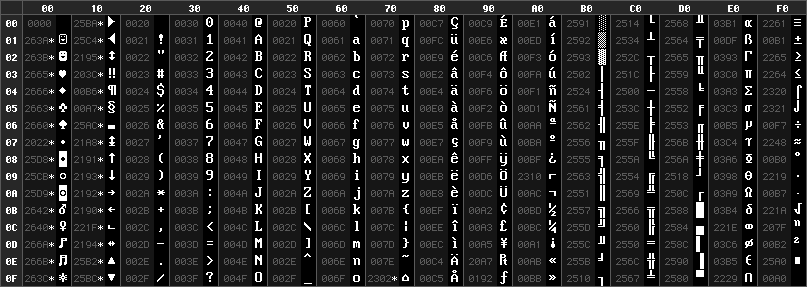
\includegraphics[width=.5\linewidth]{media/chart437.png}
  \caption[The legendary Code Page 00437.]{Code Page 00437, the IBM PC font immortalized by VGA \textit{(Source: \href{https://int10h.org/oldschool-pc-fonts/readme/}{VileR} under CCA3.0)}.}
  \label{fig:cp437}
\end{figure}

By the late 1970s, the eight-bit ``octet'' byte could be considered
dominant\footnote{\href{https://en.wikipedia.org/wiki/8-bit\_computing}{Wikipedia}
would have you believe (as of 2020-03, anyway) that the System/360 introduced
the eight-bit byte. The System/360 introduced a great many things, but
according to my own research, the IBM Stretch 7030 of 1961 used an 8-bit data
path three years prior\cite{ibmstretch}. The last major sub-octet processor
was probably the Intel 4004, and while the PDP-8 was a 12-bit machine, it
often operated on 6-bit characters.}. The very first ANSI/ISO C standard
(1989) established \texttt{CHAR\_BIT} to have a minimum value of 8\footnote{It
can have a larger value than 8, of course, and indeed does on many
DSPs\cite{cookcharbit}. POSIX does mandate that \texttt{CHAR\_BIT}==8.}. With
the high bit of an octet byte going largely unused as a parity bit, the
seven-bit character sets were rapidly expanded into a wide variety of eight-bit
character sets (sometimes mistakenly referred to as ``extended'' or ``high''
ASCII---the closest thing to ``extended ASCII'' might be the withdrawn ANSEL
ISO-IR 231 ``ANSI extended Latin''\cite{ansel}).

\begin{wrapfigure}{o}{0.4\textwidth}
\centering
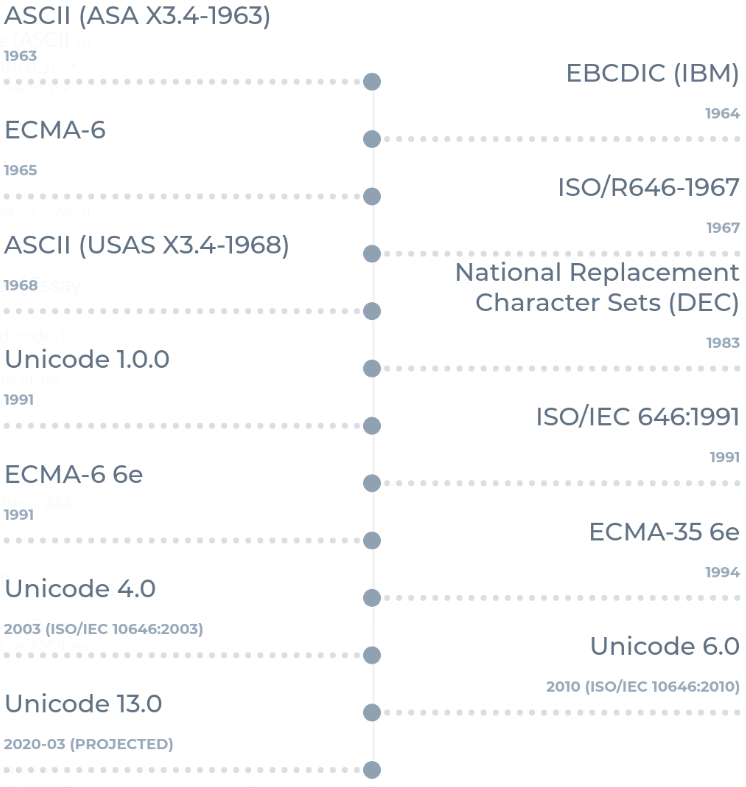
\includegraphics[width=0.5\textwidth]{media/charset-timeline.png}
\caption{Timeline of selected sets.}
\label{fig:charset-timeline}
\end{wrapfigure}

Among the better-known ASCII-derived eight-bit ``code pages'' was IBM's 00437, released
with the 5150 PC. It spread far and wide by virtue of being burned into the
ROM of IBM's MDA (9x14), CGA (8x8), EGA (8x14), and VGA (9x16) controllers.
CP437 used most of the extended space for semigraphics, mathematical symbols,
and some characters useful in the world as perceived by America circa 1981\footnote{The
 only suggestion that Asia existed as of CP437 is the ¥.}---CP437 has you
covered regarding the Dutch florin and the Spanish peseta\footnote{Which said
peseta didn't even have a symbol, just \texttt{₧}.}. It also introduced
the non-breaking space (at code 0xff). Interestingly, a melange of semigraphics
were assigned to the C0 control character code points, though these retained
their previous meanings (sometimes). All CP00437 characters have similar
glyphs in ISO 10646, though not necessarily at the same locations\footnote{A few
of the CP437 characters have multiple possible UCS equivalents;
selecting the correct one depends on context.}. Derivatives of CP437
usually jettisoned the mixed box drawing characters and some of the math
symbols to further expand alphabet coverage.

There are well over a thousand known code pages corresponding to regional,
corporate, and even private character sets, and I shall not even begin to
cover them all. There are code pages by Microsoft popularly known as the ``ANSI
code pages'' (despite not being based on any ANSI standard), and there are code
pages by IBM for Windows emulation which differ from the Windows code pages.
HTML5 requires that ``text/'' media types (that would previously have been interpreted
as ISO-8859-1) be interpreted as Windows-1252; Windows refers to
ISO-8859-1 as Windows-28591. Be glad that you are not working in the age of
8-bit character sets. This discordant cacophony gave rise to \textit{mojibake}
(文字化け [{\fontspec{DejaVu Serif}mod͡ʑibake}]), the garbled result of
mismatched character encoding and decoding\footnote{Japanese, from 文字 (moji
(character)) 化ける (bakeru (take a different form)). Russians know it as
\textrussian{кракозя́бры} (krakozyabry [{\fontspec{DejaVu
Serif}krɐkɐˈzʲæbrɪ̈}]) or sometimes \textrussian{бНОПНЯ} (bnopnjá
{\fontspec{DejaVu Serif}bnɐpˈnʲa}), while Bulgarians speak of
\textbulgarian{маймуница} (majmunica (monkey alphabet)). Serbs cut to a
characteristically Balkan chase with \textrussian{ђубре} (đubre (trash)). I
{\fontspec{DejaVu Serif}�} Unicode.}. ISO 4873\cite{iso4873} formalized a
split between control character sets (prefixed with 'C') and graphic character
sets (prefixed with 'G'); ISO 2022 formalized a baroque mechanism for shifting
between ``left'' (for handling 7-bit graphic characters) and ``right''
(for handling 8-bit graphic characters) active graphic character sets from a
selection of G0--G3. Really, be quite glad that you are not working in the age
of 8-bit character sets.

From a historical perspective, the most important eight-bit character set
is likely ISO-8859-1\cite{iso8859}, based on the Multinational Character Set
of DEC's VT220, ANSI X3.4-1986, and the C1 control code set defined in ISO 6429.
Despite being a terrible attempt at encompassing the French alphabet\footnote{French
discontent eventually resulted in the ``corrected'' ISO-8859-15, published in
1999, by which time Unicode was eight years old and no one really gave a \textit{merde}\cite{french}.},
ISO-8859-1 was directly mapped to the Basic Latin and Latin-1 Supplement blocks
of UCS, together having range 0--0xff. Thus the first 128 codepoints of both 
ISO-8859-1 (all the ISO 8859 sets, actually) and UCS are inherited from ANSI
X3.4-1986 + ISO 646's C0 + ISO 2022's universal declaration of SP (space, 0x20) and
DEL (delete, 0x7f), and the second 128 codepoints of UCS are inherited
from ISO-8859-1 + ISO 6429's C1. Only the \textit{codepoints} are equal,
however---these codepoints are not typically encoded the same way\footnote{A
notable and critical exception is UTF-8, which encodes the first 128 codepoints
the same way as ISO 646. Read on\textellipsis}.

There were also some true 16-bit and multibyte character sets, mainly in East
Asia. You might hear of Shift JIS, EUC-JP, Big5, and GB18030. How unfortunate.

\subsection{Consilience: the Universal Character Set}
\label{sec:ucs}
\begin{figure}[!htb]
  \centering
  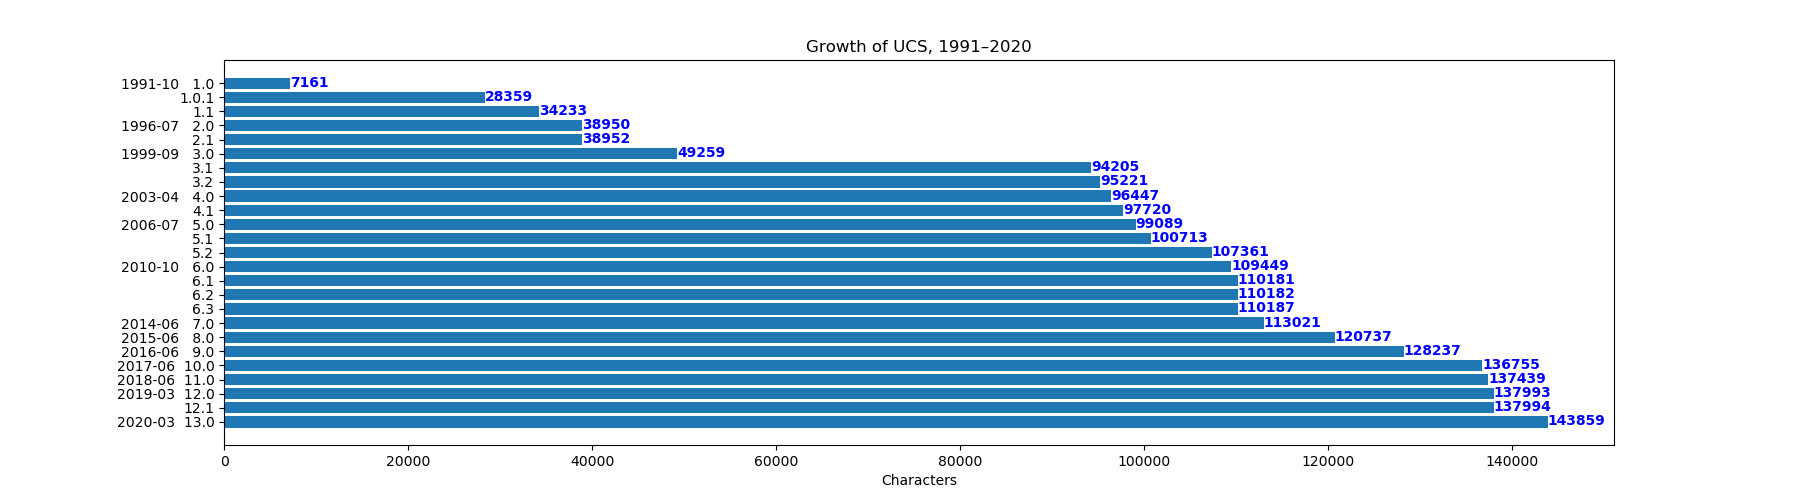
\includegraphics[width=1.1\linewidth]{media/unicode-growth.png}
  \caption{2020's Unicode 13.0 ships 143,859 character definitions.}
  \label{fig:unicodegrowth}
\end{figure}

\begin{table}[!htb]
  \begin{center}
    \begin{tabular}{ |c|l| }
      \hline
      Principle & Statement \\
      \hline
      \hline
      Universality & \makecell[l]{The Unicode Standard provides a single, universal repertoire.} \\
      \hline
      Efficiency & Unicode text is simple to parse and process. \\
      \hline
      Characters, not glyphs & The Unicode Standard encodes characters, not glyphs. \\
      \hline
      Semantics & Characters have well-defined semantics. \\
      \hline
      Plain text & Unicode characters represent plain text. \\
      \hline
      Logical order & The default for memory representation is logical order. \\
      \hline
      Unification & \makecell[l]{The Unicode Standard unifies duplicate characters within scripts\\across languages.} \\
      \hline
      Dynamic composition & Accented forms can be dynamically composed. \\
      \hline
      Stability & \makecell[l]{Characters, once assigned, cannot be reassigned and key properties\\are immutable.} \\
      \hline
      Convertibility & \makecell[l]{Accurate convertibility is guaranteed between the Unicode Standard\\and other widely accepted standards.} \\
      \hline
    \end{tabular}
  \end{center}
  \caption[The ten Unicode design principles.]{The 10 Design Principles of Unicode (Unicode Core Specification §2.2\cite{unicode}).}
  \label{table:ucsdesign}
\end{table}
The Universal Character Set (ISO 10646\footnote{Note that this is 10,000 more than ISO 646. Cute?},
the character set underlying Unicode) was introduced to resolve these problems,
as a ``unique, universal, and uniform character encoding''\cite{unicodehistory}. The
Unicode Consortium traces its origin to Joe Becker's paper, ``Unicode 88''\cite{unicode88}.
Often in these early documents, UCS is described as a ``16-bit character set''.
This is perhaps partially responsible for the widespread misconception that UTF-16\cite{rfc2781}
can encode all UCS code points in a single 16-bit unit. 16 bits are sufficient
to encode any given UCS \textit{plane} of up to 65,536 code points, and indeed a great
many languages are contained within the first UCS plane, the Basic Multilingual
Plane (0x0--0xffff). There are a total of 17 planes available in
UCS\footnote{Once upon a time, these other sixteen planes were known as the
Astral Planes\cite{astralplanes}.}, however, and UTF-16 requires two code
units to encode points from these other 16 planes (0x10000--0x10ffff).

\begin{table}[!htb]
  \begin{center}
    \begin{tabular}{ |c|c|l| }
      \hline
      Plane & ID & Purpose \\
      \hline
      \hline
      Basic Multilingual & 0 & Common-use characters for modern and historical scripts. \\
      \hline
      Supplementary Multilingual & 1 & Spillover from BMP. \\
      \hline
      Supplementary Ideographic & 2 & CJK spillover from BMP. \\
      \hline
      Supplementary special-purpose & 14 & Format control spillover. \\
      \hline
      Supplementary Private Use A & 15 & Local semantics. \\
      \hline
      Supplementary Private Use B & 16 & Local semantics. \\
      \hline
    \end{tabular}
  \end{center}
  \caption[The six named UCS planes.]{The six named UCS planes (Unicode Core Specification §2.8\cite{unicode}).}
  \label{table:ucsplanes}
\end{table}

Below the plane comes the \textit{block}, a range of between 16 and 65,536 related
code points, always starting on a 16-codepoint boundary. A block is merely a
convenience for reference. Each codepoint belongs to one and only one block.
As mentioned earlier, the first 256 code points of UCS (making up the first two
blocks) are taken from ISO-8859-1, plus DEL and the control character classes
C0 and C1.
\begin{figure}[!htb]
\centering
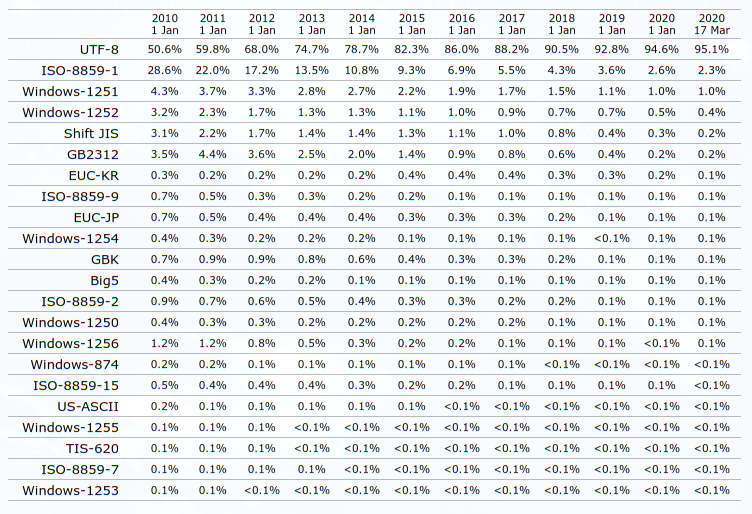
\includegraphics[width=0.5\textwidth]{media/yearly-charsets.png}
\caption{Charsets served over the last decade on the Web \textit{(source: \href{https://w3techs.com/technologies/history\_overview/character\_encoding/ms/y}{W3Techs})}.}
\label{fig:charsetuse}
\end{figure}

\subsection{Fixed-width fonts ain't so fixed}
Notcurses assumes that all glyphs occupy widths which are an integral multiple
of the smallest possible glyph's cell width (aka a ``fixed-width font'').
Unicode introduces characters which generally occupy two such cells, known as
wide characters (though in the end, width of a glyph is a property of the
font). It is not possible to print half of such a glyph, nor is it generally
possible to print a wide glyph on the last column of a terminal.

Notcurses does not consider it an error to place a wide character on the last
column of a line. It will obliterate any content which was in that cell, but
will not itself be rendered. The default content will not be reproduced in such
a cell, either. When any character is placed atop a wide character's left or
right half, the wide character is obliterated in its entirety. When a wide
character is placed, any character under its left or right side is annihilated,
including wide characters. It is thus possible for two wide characters to sit
at columns 0 and 2, and for both to be obliterated by a single wide character
placed at column 1.

Likewise, when rendering, a plane which would partially obstruct a wide glyph
prevents it from being rendered entirely. A pathological case would be that of
a terminal $n$ columns in width, containing $n-1$ planes, each 2 columns wide.
The planes are placed at offsets $[0\ldots n-2]$. Each plane is above the plane to
its left, and each plane contains a single wide character. Were this to be
rendered, only the rightmost glyph would be visible!

Finally, fonts and font engines which yield glyphs wider (or narrower) than
\texttt{wcwidth()} would lead Notcurses to believe can cause problems. It is
best to avoid EGCs known to be very wide, or to avoid fonts which generate very
wide glyphs. Some examples are shown in Figure~\ref{fig:wideglyphs}.

\begin{figure}[!htb]
\centering
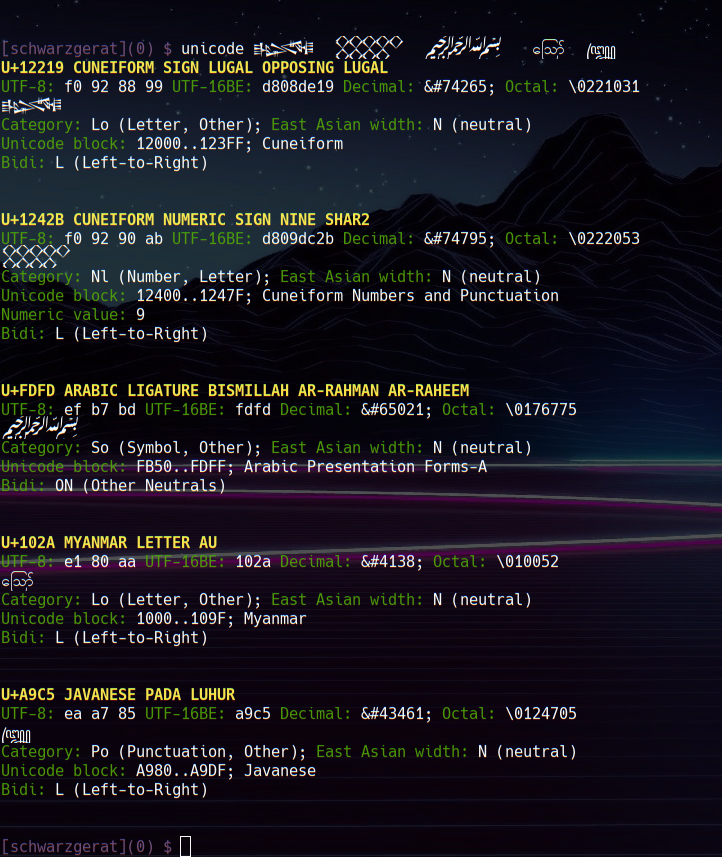
\includegraphics[width=1\linewidth]{media/wide-unicode.png}
\caption[Some very wide Unicode glyphs.]{Some very wide Unicode glyphs (font: Hack 10)}
\label{fig:wideglyphs}
\end{figure}

\subsection{Emoji}
According to Unicode Standard Annex \#51\cite{annex51}, emoji are ``pictorial
symbols that are typically presented in a colorful cartoon form and used
inline in text. They represent things such as faces, weather, vehicles and
buildings, food and drink, animals and plants, or icons that represent
emotions, feelings, or activities.''
Don't blame me, mang; I didn't do it. Emoji (Japanese 絵文字えもじ ([{\fontspec{DejaVu Serif}emodʑi}]),
絵 (picture) and our old friend 文字 (moji (character)) emerged from Japan
in the late 90s, and by June 2019 they were in the Oxford Fucking Dictionary of
the English Language\cite{oedgay}---sorry, I get kinda touchy about the OED.
Emoji represent, by far, the most kibbitzed-upon, politicized, arbitrary
element of Unicode; for us, they are also the most dangerous. Presentation of
emoji is rivaled only by bidirectional text for variation across platforms.

Some Unicode ``emoji'' support only a textual presentation (\texttt{text-only}),
while some support both (with different defaults
(\texttt{text-default}/\texttt{emoji-default}) for different characters).
Selecting the presentation can sometimes be done by following the base with
\texttt{U+FE0E VARIATION SELECTOR-15} (for text) or \texttt{U+FE0E VARIATION
SELECTOR-16} (for emoji). The full data on such things is in the
Unicode-adjacent ``Data files for emoji characters'', but how closely your
local implementation will conform this week is generally unknowable.

When using the textual presentation, emoji can be arbitrarily colored according
to the standard Notcurses mechanisms. Emoji presentation will typically make use
of its own colors (the background color will usually be honored, in my
experience). The Fitzpatrick dermatological scale has been adopted for modifying
the skin tone of base glyphs via Zero-Width-Joiner (ZWJ) sequences. Characters
which can be so modified are designated with the \texttt{Emoji\_Modifier\_Base}
property, and can be affected by characters with the \texttt{Emoji\_Modifier}
property. Both (and the ZWJ character) are part of the same EGC. ``Standard'' ZWJ
sequences are described as ``Recommended for General Interchange'' (RGI) in
the Unicode data files.

Official Unicode support for the concept of emoji was added in Unicode 6.0, but
some earlier characters have been retroactively recognized as emoji, reaching
all the way back to the 23 Zapf Dingbats of Unicode 1.0. Unicode 5.2 added
88 symbols for conformance with the Japanese Association of Radio
Industries and Businesses (ARIB). The remaining 608 characters necessary to
cover various Japanese mobile carriers were added to 6.0 (and indeed their
definitions are given in terms of the Shift-JIS encoding\cite{emojiversions}).
Unicode 6.1 added the concept of emoji presentation.

Google, Apple, and other Californian megacorporations think
\xelatexemoji{1f52b-200e} is the best representation for
\xelatexemoji{1f52b-200d} \texttt{U+1F52B PISTOL} (I personally like
\xelatexemoji{1f52b}). That'll be important for things like
{\fontspec{Symbola}{🐊🔫👮}}, an example used in \#51 to illustrate the
importance of maintaining pictograph direction. It's a madhouse out there.

You might have seen what appeared to be emoji flags of the world. The Unicode
Consortium, in their wisdom, wanted nothing to do with such geopolitical
questions. Instead, the 26 ``Regional Indicator Symbols``---one for each
letter of the ISO basic Latin alphabet\cite{iso646}---can be used to encode
ISO 3166-1\cite{iso3166} two-letter country codes\cite{darkcorners}. Some fonts contain flag
glyphs, and some layout engines will map pairs of these symbols to flags. The
UCS \textit{does not} contain national ``flag emoji'' (it does have some other
flags, though---see Table~\ref{table:flags}\footnote{Using a green block,
it is possible to generate the flag of the Great Socialist People's Libyan Arab Jamahiriya through 2011.}).

\begin{table}[!htb]
  \centering
  \begin{tabular}{|l|l|l|}
  \hline
  Character & Version & Comments \\
  \hline
  \hline
  🎌 U+1F38C CROSSED FLAGS & Unicode 6.0 & why Japanese crossed flags? \\
  \hline
  🏁 U+1F3C1 CHEQUERED FLAG & Unicode 6.0 & ``chequered'' whatever \\
  \hline
  🏳 U+1F3F3 WAVING WHITE FLAG & Unicode 7.0 & surrender! \\
  \hline
  🏴  U+1F3F4 WAVING BLACK FLAG & Unicode 7.0 & the Nick Black flag amirite \\
  \hline
  🚩 U+1F6A9 TRIANGULAR FLAG ON POST & Unicode 6.0 & suspiciously golf-related \\
  \hline
  \end{tabular}
  \caption{Flags in Unicode.}
  \label{table:flags}
\end{table}

There are also official and non-official EGCs that commonly render flags, including
the Jolly Roger (U+1F3F4, U+2620, \xelatexemoji{1f3f4-200d-2620-fe0f}),
Gilbert Baker's rainbow flag (U+1F3F3, U+1F308, \xelatexemoji{1f3f3-200d-1f308+fe0f}) and Monica Helms's
transgender flag (U+1F3F3, U+26A7, \xelatexemoji{1f3f3-200d-26a7-fe0f}).
If you don't like the latter, you can always throw U20E0 COMBINING ENCLOSING
CIRCLE BACKSLASH atop it:\xelatexemoji{1f3f3-200d-1f308-20e0-fe0f}. It's a big Unicode tent, and there are plenty
of EGCs for everybody.

The downside of using such complexly combined EGCs is of course that what's
intended to be a single EGC can be broken into multiple EGCs by the font
rendering system. Suddenly, instead of \xelatexemoji{1f3f4-200d-2620-fe0f}
you've got an inscrutable \texttt{🏴☠}. To add insult to injury, this will
almost certainly screw up geometry through the end of the line, since Notcurses
will have an incorrect concept of the cursor's horizontal position. This
assumes that the font in use has even the basic component glyphs---in the very
limited Linux console font, it's unlikely that anything good can come of using
composed emoji. When used properly under aligned stars, however, emoji can make
your TUI pop like nothing else.

Some applications map emoticons to emoji. This is not performed at the terminal
level for any terminal of which I am aware, so if you want this feature, you'll
need effect it yourself. Notcurses provides no support for this, because I
think it's dumb. There is no concept of emoticons in Unicode.

\subsection{Stupid Unicode tricks}
Perhaps the single most useful Unicode character is U+2580 UPPER HALF BLOCK
(\texttt{▀}), or alternatively its inverse U+2584 LOWER HALF BLOCK
(\texttt{▄}). By using these together with both a foreground and background,
it is possible to treat a region of cells as a ``framebuffer'' having
vertical resolution twice the number of occupied lines, and perhaps more importantly
having a cell aspect ratio of 1:1. With this technique, it's trivial to blit
RGBA as provided by e.g. image decoders and get good results (this is exactly
what's done in Notcurses's media layer, see Chapter~\ref{sec:libav}). A smart
implementation will, when possible, replace a HALF BLOCK plus two RGB specifications
with U+2588 FULL BLOCK and a single foreground RGB. A smarter implementation
still will, when possible, replace a FULL BLOCK with a space and a single
background RGB\footnote{This optimization is not possible when, for instance,
the alphas are anything other than \texttt{CELL\_ALPHA\_OPAQUE}.}, though this
optimization saves only 2 bytes compared to the dozen or so saved by eliding
an RGB escape. Notcurses effects both optimizations.

\begin{figure}[!htb]
    \centering
    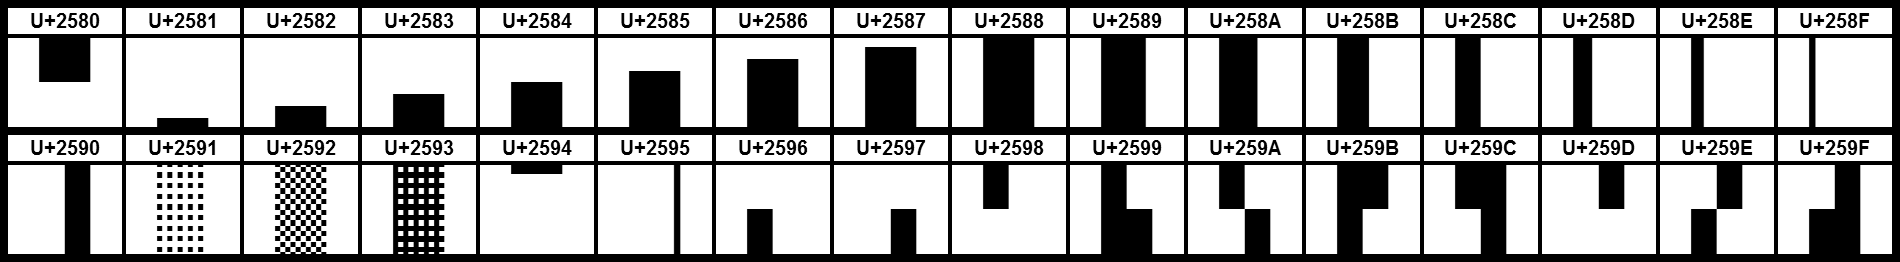
\includegraphics[width=.75\linewidth]{media/blockelements.png}
    \caption{Unicode 13.0 Block Elements \textit{(source: \href{https://commons.wikimedia.org/wiki/File:UCB_Block_Elements.png}{Antonsusi} under CCA3.0)}.}
    \label{fig:blockelements}
\end{figure}

Unfortunately, it's difficult to take this technique any further. There are
U+258C LEFT HALF BLOCK (\texttt{▌}) and U+2590 RIGHT HALF BLOCK (\texttt{▐}):
they exacerbate the character cell aspect ratio problem, but can still be
useful for rendering certain surfaces in tall, thin geometries. A single cell
can be divided up to 8 ways using the eighths blocks, but only being able to
supply two colors (not to mention the resulting aspect ratio) means this can't
be easily used for 8x resolution. There are three incompletely-filled shades of
U+2588 FULL BLOCK, which could conceivably be used to increase the color range
by a factor of 4, but the 24-bit RGB space is already pretty large---resolution
is a much more precious resource.

Those readers who remember Code Page 437 might recall 0xFD, a ``middle half
block''. Given a constant background, this can be used with the other two
half blocks to increase ``vertical resolution'' by a factor of 3 (imagine a
tank drawn with upper, middle, and lower half blocks moving on a monochromatic
background). Well, that character was actually ``Solid Square/Histogram/Square Bullet''
in the CP437 definitions\cite{cp437}, and lives on as U+25A0 BLACK SQUARE (\texttt{■}).
Despite its name, it will take on the foreground color.

It might be useful to use the quadrant characters to effect a 2x2 resolution
doubling. The quadrants cannot yield a lossless reproduction for any 2x2 block
that uses more than two colors, but it might be useful to interpolate given the
small total number of possible colors. Some graduate student ought look
into this.

It is possible to use the Braille Patterns at U+2800 to get an 8x increase in
resolution, at the cost of having only two colors available per 2x4 ``8-pixel''
cell (and looking like blotter paper, depending on the font). This can be an
excellent solution for e.g. graphing, especially vertical histograms. By
inspecting Figure~\ref{fig:braille}, it ought be clear that the 8 areas
map to distinct bits: counterclockwise from the upper left, the bits are 1, 2,
4, 64, 128, 32, 16, 8. This odd ordering is due to true braille only being a
6-bit (64 character) character set; this way, real braille maps to the first
64 codepoints.

\begin{figure}[!htb]
    \centering
    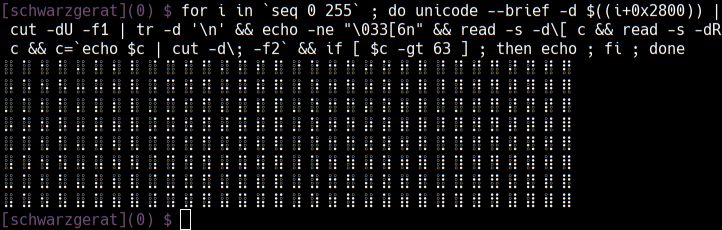
\includegraphics[width=1\linewidth]{media/braille-unicode.png}
    \caption{Unicode Braille characters.}
    \label{fig:braille}
\end{figure}

Certain sets of Unicode characters form cyclic groups. These can be useful for
simple, single-cell animations, e.g. work-indicating ``spinners''. I've isolated
some of these groups in Table~\ref{table:cyclics}. Smaller groups can usually
be isolated from larger groups: as an example, the eight-way HALF-SQUARE cycle
yields two four-way subcycles and four two-way subcycles.

\begin{table}[!htb]
  \centering
  \begin{tabular}{|l|l|l|}
    \hline
    Size & Glyphs & Comments \\
    \hline
    \hline
    2 & {\fontspec{Symbola}▱▰} & \makecell[l]{Parallelogram. You can get a kinda\\ neat ``barber-pole'' effect by alternating each period.} \\
    \hline
    4 & \textbackslash{}|/- & Approximate, but works even under ASCII. \\
    \hline
    4 & {\fontspec{Symbola}◰◳◲◱} & Note that they're out of order \\
    \hline
    6 & {\fontspec{Symbola}🞯🞰🞱🞲🞳🞴} & Five-spoked asterisk \\
    \hline
    6 & {\fontspec{Symbola}🞵🞶🞷🞸🞹🞺}  & Six-spoked asterisk \\
    \hline
    5 & {\fontspec{Symbola}🞻🞼🞽🞾🞿} & \makecell[l]{Fuck your seven-spoked asterisk, fuck expecting six \\eight-spoked asterisks, and fuck you too.} \\
    \hline
    8 & {\fontspec{Symbola}◧◩⬒⬔◨◪⬓⬕} & Some fonts have different sizes. Why? Ugh. \\
    %8 & \texttt{◧◩⬒⬔◨◪⬓⬕} & Some fonts have different sizes. Why? Ugh. \\
    \hline
    10 & {\fontspec{Symbola}🞌🞍🞎🞏🞐🞑🞒🞓🞔🞕🞖} & The first two are maybe cheating. \\
    \hline
  \end{tabular}
  \caption{Just a few of Unicode's many cyclic groups.}
  \label{table:cyclics}
\end{table}

Certain transformations can be safely applied to the full Latin alphabet
(see Figure~\ref{fig:unicodeweird} for more, some of which I couldn't
realize in \XeLaTeX).

\begin{denseitemize}
\item{{\fontspec{Unifont}ⓦⓔ ⓒⓐⓝ ⓟⓤⓣ ⓞⓤⓡ ⓣⓔⓧⓣ ⓘⓝ ⓒⓘⓡⓒⓛⓔⓢ}}
\item{stretttch text with fullwidth}
\item{{\fontspec{DejaVu Serif}𝕞𝕒𝕥𝕙 𝕕𝕠𝕦𝕓𝕝𝕖 𝕤𝕥𝕣𝕦𝕔𝕜, 𝕗𝕠𝕣 𝕥𝕙𝕠𝕤𝕖 𝕨𝕙𝕠 𝕨𝕚𝕤𝕙 𝕥𝕠 𝕝𝕠𝕠𝕜 𝕝𝕚𝕜𝕖 ℝ\^𝕟}}
\end{denseitemize}

Others can be performed on a good chunk of Latin script, but are incomplete:

\begin{denseitemize}
\item{{\fontspec{DejaVu Serif}ᴘᴀᴄᴋ ᴍʏ ʙᴏx ᴡɪᴛʜ ꜰɪᴠᴇ ᴅᴏᴢᴇɴ ʟɪqᴜᴏʀ ᴊᴜɢꜱ (smallcaps)}}
\item{{\fontspec{DejaVu Serif}ₚₐcₖ ₘy bₒₓ wᵢₜₕ fᵢᵥₑ dₒzₑₙ ₗᵢqᵤₒᵣ ⱼᵤgₛ (subscripts)}}
\item{{\fontspec{DejaVu Serif}ᴾᵃᶜᵏ ᵐʸ ᵇᵒˣ ʷⁱᵗʰ ᶠⁱᵛᵉ ᵈᵒᶻᵉⁿ ˡⁱqᵘᵒʳ ʲᵘᵍˢ (superscripts)}}
\item{{\fontspec{DejaVu Serif}dɐɔʞ ɯʎ qox ʍıʇɥ ɟıʌǝ pozǝu ןıbnoɹ ɾnƃs (inverted)}}
\item{{\fontspec{DejaVu Serif}ꟼAↄk mY dox wiTH ꟻivɘ bozɘᴎ lipUoᴙ jUgꙅ (reversed)}}
\end{denseitemize}

\begin{figure}[!htb]
    \centering
    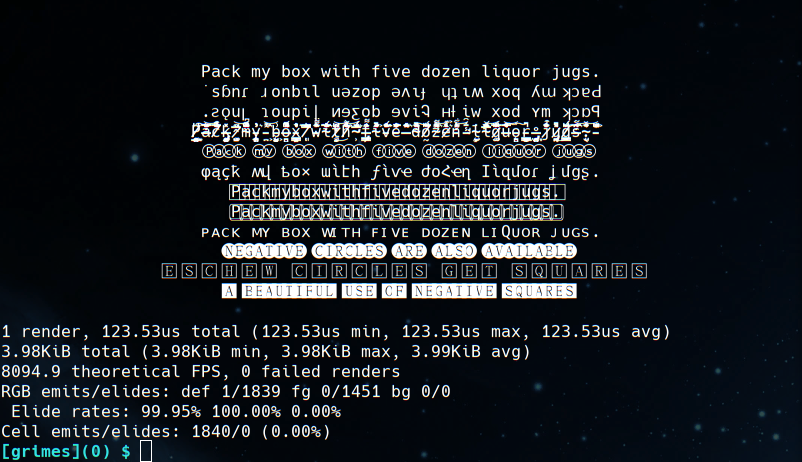
\includegraphics[width=.75\linewidth]{media/unicode-weird.png}
    \caption{A pangram using a variety of Unicode texts.}
    \label{fig:unicodeweird}
\end{figure}

``Pseudoalphabets'' by the thousand exist. These simply substitute glyphs for
others of which they are more or less suggestive. There's no real rhyme or
reason behind these pseudoalphabets, but they can be useful if you need a
different ``font''. Some examples are shown in Figure~\ref{fig:pseudoalphabets}.

\begin{figure}[!htb]
    \centering
    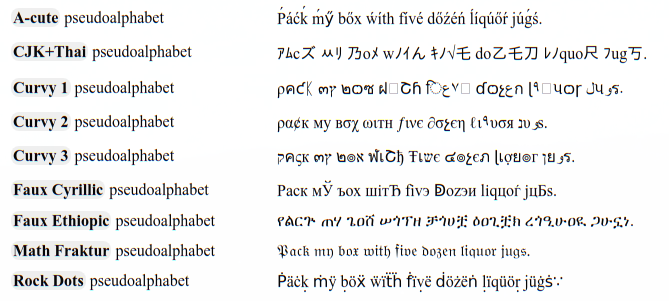
\includegraphics[width=.75\linewidth]{media/pseudoalphabets.png}
    \caption{Some of ``Eli the Bearded'''s pseudoalphabets from \url{http://qaz.wtf/u/}.}
    \label{fig:pseudoalphabets}
\end{figure}

Finally, we can't speak of stupid Unicode tricks without mentioning
\textit{zalgo}: \texttt{i̸̬̦͙̒̌̓͝n̴͛̓͋̈́͂̇̑̅̕e̵̎̈́̎̀̐̓͆͘͝l̴̠͛͂̃́̅̄̚͝u̷̾́̄̇́̎͂̚͝c̴̡̟̜̉̈́̋͂̈́̎t̵́͊̂̑̑̇̒̃̄å̵̰͎̫̅̿̏͂̽b̷̛͋̎́͛́͋̈͌l̷̰͎̫͐̑̈͛͆͝e̴̱̋̾̃̒̏͘͘̕m̸̆͋͌̍̉͆͌͛̓ȍ̷̡̜̭͙̞̣̎̚d̴̐̃͆̈́̽̔̐̀͝ä̸́̑̐̒͊̔̾́̕l̶̨̡̙̳̭̮̠̼͝i̷̋̆̌̿̎̃̋̚̚ṯ̷̱̫̺͗͒̔͆̄ẏ̷̡̛̮͈͑̓́͊ȏ̵͋̅́̋͒̐̇͝f̸̛̃͐͒̈̾̆̕͠t̶͈̱̠͋̑̊̿̇͘h̷̰͚̳̳̤͗̓͗̄e̴͇͙̜̿͐́̎̌͘ṽ̶̌̈́́́̈́͌͂͘i̷̛͊̒̏̄̀̅͠͝s̸̯̘͍̝͓̈́ͅͅì̵̃͊̇͗̄̋̇͘b̷̃̎̓͛̊̾͘̚̚l̶̯̼͎͉̎͛̆͠e̷̙͊̇̿͗̃͊̓́}. Dump enough
diacritics into an EGC, and the result is a somewhat Cthulhian garble (it's not
quite \textit{squamous}, and I wouldn't go so far as to call it
\textit{eldritch}, but I suppose it's \textit{unheimlich}). Investigating zalgo
led down a Reddit hole of madness; I mention it only for completeness, and as
an excuse to include Figure~\ref{fig:zalgo}.

\begin{figure}[H]
    \centering
    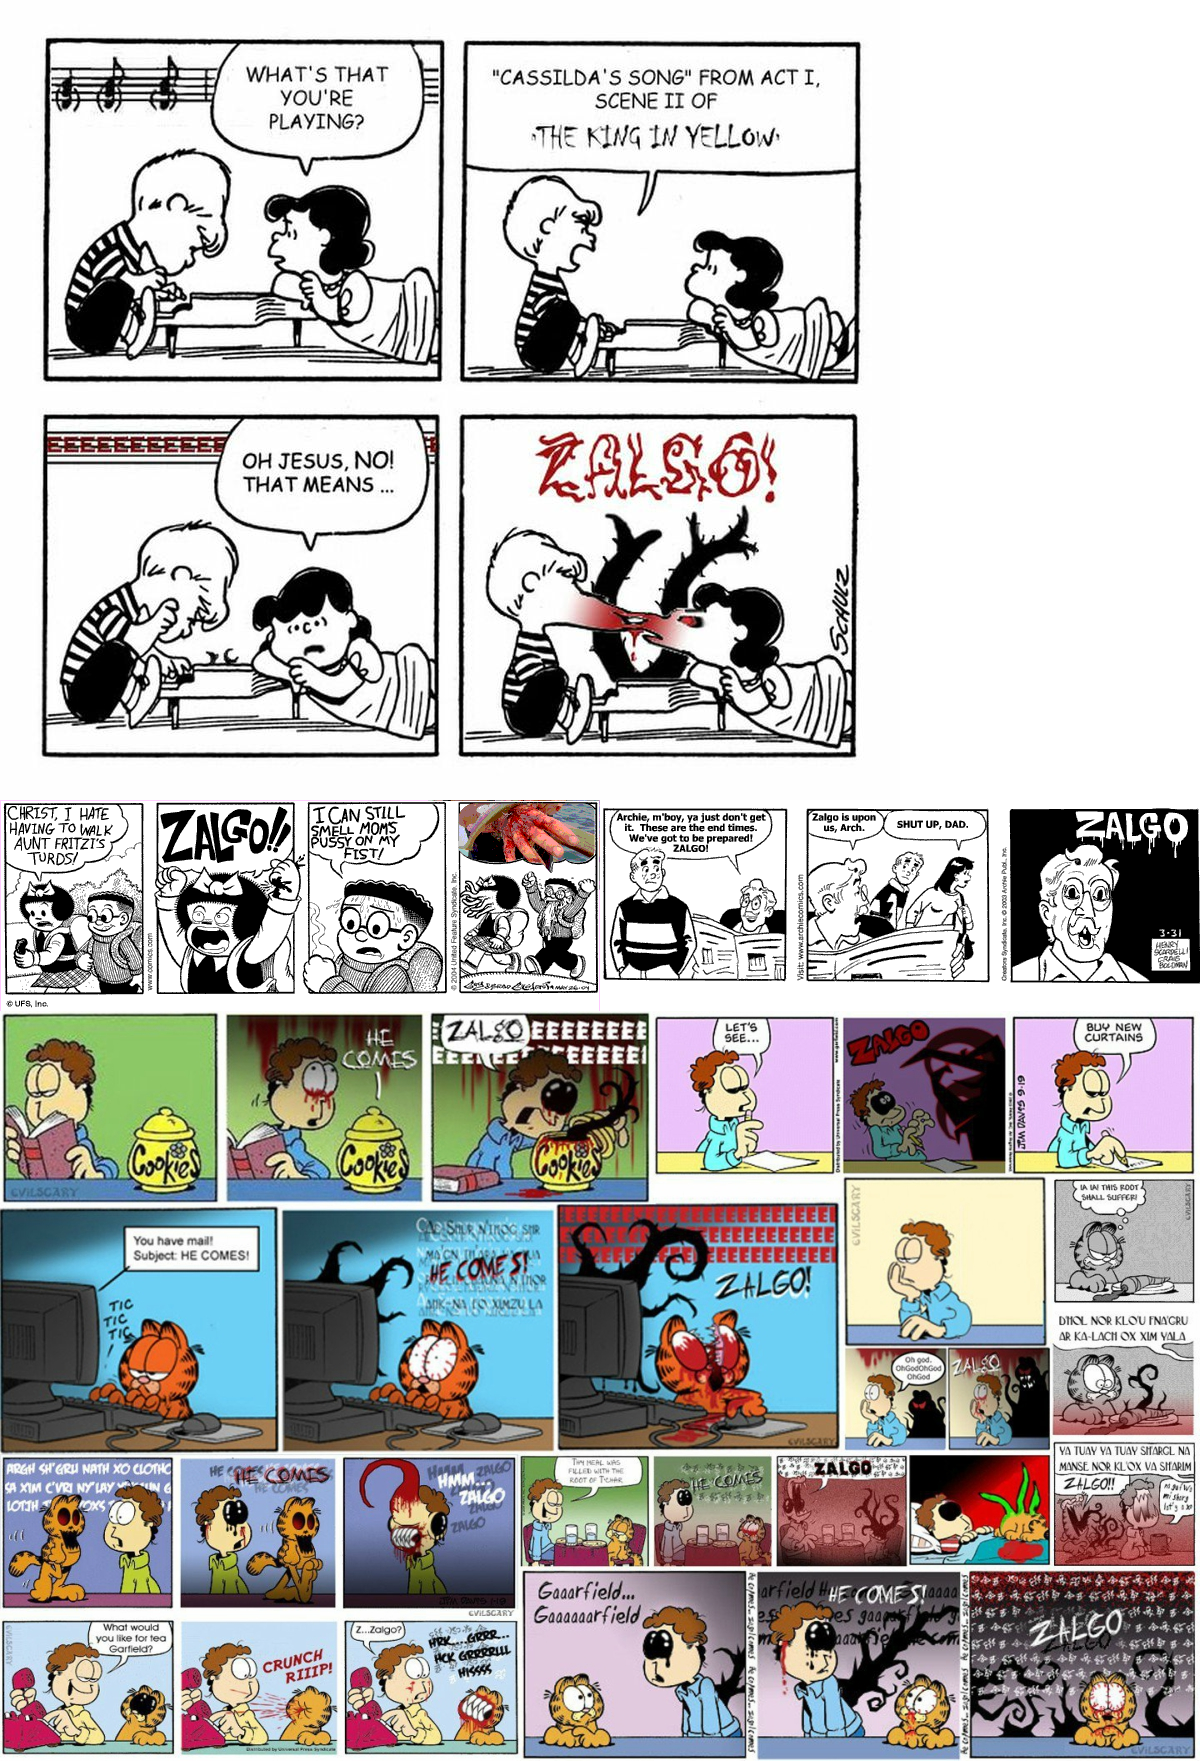
\includegraphics[width=.5\linewidth]{media/zalgo.png}
    \caption{Past, present, future, all are one in Yog-Sothoth.}
    \label{fig:zalgo}
\end{figure}

\subsection{UTF-8}
Unicode Technical Report \#17\cite{annex17} defines seven official Unicode
character encoding schemese: UTF-8, UTF-16, UTF-16BE, UTF-16LE, UTF-32, UTF-32BE,
and UTF-32LE. What a wealth of encodings! How is one to choose? The -16BE and
-16LE forms are simply UTF-16 with a known byte order; a UTF-16 stream can
(optionally!) be prefixed with a Byte-Order Mark, at which point the stream
reduces to -16LE or -16BE (in the absence of a BOM, the best advice is to follow
your heart). UTF-32 breaks down the same way. This question of endianness arises
from the fact that UTF-16 and UTF-32 are coded in terms of 16- and 32-bit units.
UTF-8, being coded in terms of individual bytes, has no need to define byte order.

``Well, that BOM sounds kinda annoying,'' I hear you asking. ``What other
advantages are offered by UTF-8?'' Remember how ANSI X3.4-1986 maps precisely
to the first 128 characters of UCS? UTF-8 (and \textit{only} UTF-8, of
the official encodings) \textit{encodes} these 128 characters the same as
US-ASCII! Boom! Every ASCII document you have---including most source code,
configuration files, system files, etc.---is a perfectly valid UTF-8 document.
Furthermore, UTF-8 \textit{never encodes non-ASCII characters to the ASCII
bytes}. So an arbitrary UTF-8 document may have plenty of high-bit bytes that
your ASCII-aware, POSIX-locale program doesn't understand, but it never sees
a valid ASCII character where one wasn't intended. UTF-8 encodes ASCII's 0--0x7f
to 0--0x7f, and otherwise never produces a byte in that range. This includes
the all-important null character 0---Boom! Every nul-terminated C string is a
valid UTF-8 string. Every UTF-8 string can be passed through standard C APIs
cleanly, and they'll more or less work. It's furthermore self-synchronizing.
If you pick up a UTF-8 stream in the middle, you know after reading a single
byte whether you're in the middle of a multibyte character.

``Sweet! What's the catch? Does it waste space?'' RFC 3629\cite{rfc3629}
limits UTF-8's range to the $17*2^{16}$-ary code space of UCS, in which case
the maximum length of a single UTF-8-encoded UCS code point is four bytes\footnote{You
might hear six bytes, and indeed ISO/IEC 10646 specifies six bytes to handle
up through U+7FFFFFFF\textellipsis but only defines UCS to cover 17 planes.
Verify your \texttt{wctomb(3)} rejects inputs in excess of 0x10ffff before
exploiting RFC 3629's tighter bound.}. It's thus always as or more efficient
than UCS-32. When the ASCII characters are used, UTF-8 is more efficient than
either UTF-16 or UTF-32. Only for streams utterly dominated by BMP codepoints
requiring three or more bytes from UTF-8 can UTF-16 encode more efficiently.

``Sweet! What's the catch? Is it super slow?'' UTF-32, it is true, allows you
to index into a string by character in O(1) (UTF-16 \textit{does not}, unless
you're only dealing with BMP strings). UTF-32 also allows you to compute the
bytes necessary for encoding in O(1), given the number of Unicode codepoints,
but that's only because it's wasteful; if you're willing to be similarly
wasteful, you can do the same calculation with UTF-8 (and then trim any wastage
at the end, if you wish). Any advantage UTF-32 might hold in lexing simplicity
is likely a wash when UTF-8's usual space efficiency is taken into account,
owing to more effective use of cache and memory bandwidth. Nope, it's not slow.
\textbf{Always interoperate in UTF-8 by default.}

UTF-16 is some truly stupid shit, fit only for jabronies. It only ever passed
muster because people thought UCS was going to be a sixteen-bit character set.
The moment a second Plane was added, UTF-16 ought have been shown the door.
There's an argument to be made for ripping it from the pages of books
in your local library. If you must work on a UTF-16
system, use UTF-16 at the boundary, and then keep it around as UTF-32 or UTF-8.
Always interoperate---including writing files---in UTF-8 by default.

There are a dozen-odd similarly-named encodings which are useful for nothing
but trivia. UCS-2 was UTF-16, but for only the BMP. UCS-4 is just UTF-32. UTF-7
is a seven-bit-clean UTF-8\footnote{The primary seven-bit-clean media of the
modern era is probably email sent without a MIME transfer encoding.}. UTF-1 is UTF-8's older, misshapen sister, locked away from
sight in the attic. UTF-5 and UTF-6 were proposed encodings for IDN, but
Punycode was selected instead. WTF-8 extends UTF-8 to handle invalid UTF-16
input. BOCU-1 and SCSU are compressing encodings that
don't compress as well as gzipped UTF-8. UTF-9 and UTF-18 were jokes. Is
UTF-EBCDIC a thing? Of course UTF-EBCDIC is a thing\footnote{Perhaps the
most cursed thing I'm aware of in computing is
``UTFE'', a variable-length UCS encoding that somehow requires six bytes
sometimes, is used exclusively on EBCDIC platforms, and furthermore exclusively
only on (drum roll)\textellipsis. EBCDIC. ORACLE. DATABASES. Ave Satanas! Also receiving
votes: Threaded INTERCAL, non-Postfix mail servers, old-skool XFree86 configuration
files with the modeline bullshit, ActiveX controls, ``WebNFS'', Perl.}.

The one place where you won't interoperate with UTF-8 is for domain name lookup,
when converting IDNA into the LDH subset of ASCII. If you're interested,
consult RFC 3492, and Godspeed.

\begin{figure}[!htb]
    \centering
    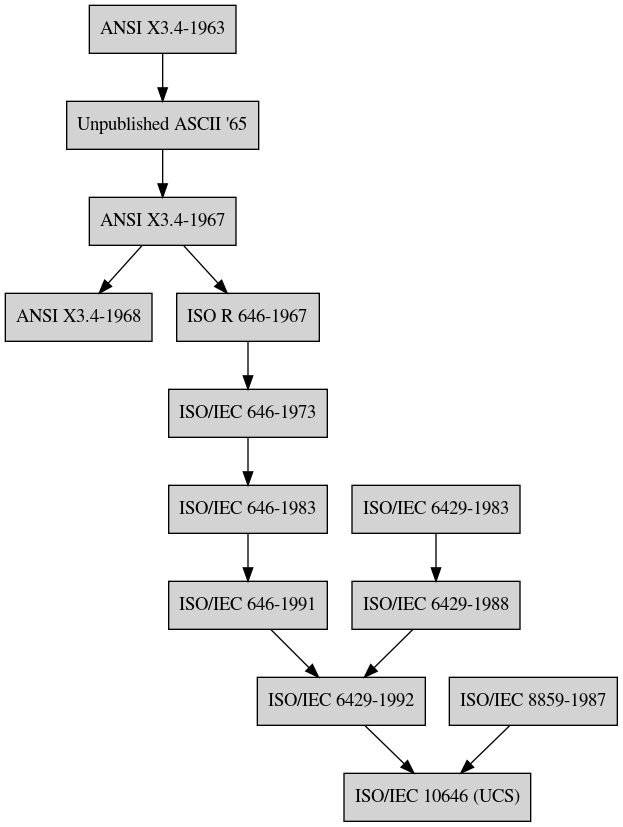
\includegraphics[width=.75\linewidth]{media/control-char-standards.png}
    \caption{Flow of control characters through historic standards.}
\end{figure}

\cleardoublepage
%%%%%%%%%%%%%%%%%%%%%%%%%%%%%%%%%%%%%%%%%%%%%%%%%%%%%%%%%%%%%%%%%%%%%%%%
